\section{Anwendungsfälle}


Im folgenden Abschnitt werden für die drei Visualisierungen jeweils Anwendungsfälle vorgestellt und diskutiert, die sich auf die Bewertung von Gebrauchtwagenanzeigen beziehen. Die Zielgruppe (Gebrauchtwagenhändler) hat den Bedarf, die besten Angebote sowie relevante Attribute zu identifizieren.

Die Anwendungsaufgaben der Zielgruppe konzentrieren sich darauf, Gebrauchtwagenanzeigen anhand verschiedener Kriterien zu bewerten. \\
Dabei haben Gebrauchtwagenhändler innerhalb des Verkaufsprozesses eines Autos mehrere Kontaktpunkte mit Gebrauchtwagenplattformen, denn sie verkaufen dort nicht nur ihre eigenen Wagen, sondern sourcen ihre Ware meist auch auf diesen Plattformen. Dieser Prozess ist als Geschäftsprozess in Abbildung \ref{fig:business-process} dargestellt. \\

\begin{figure}[H]
    \centering
    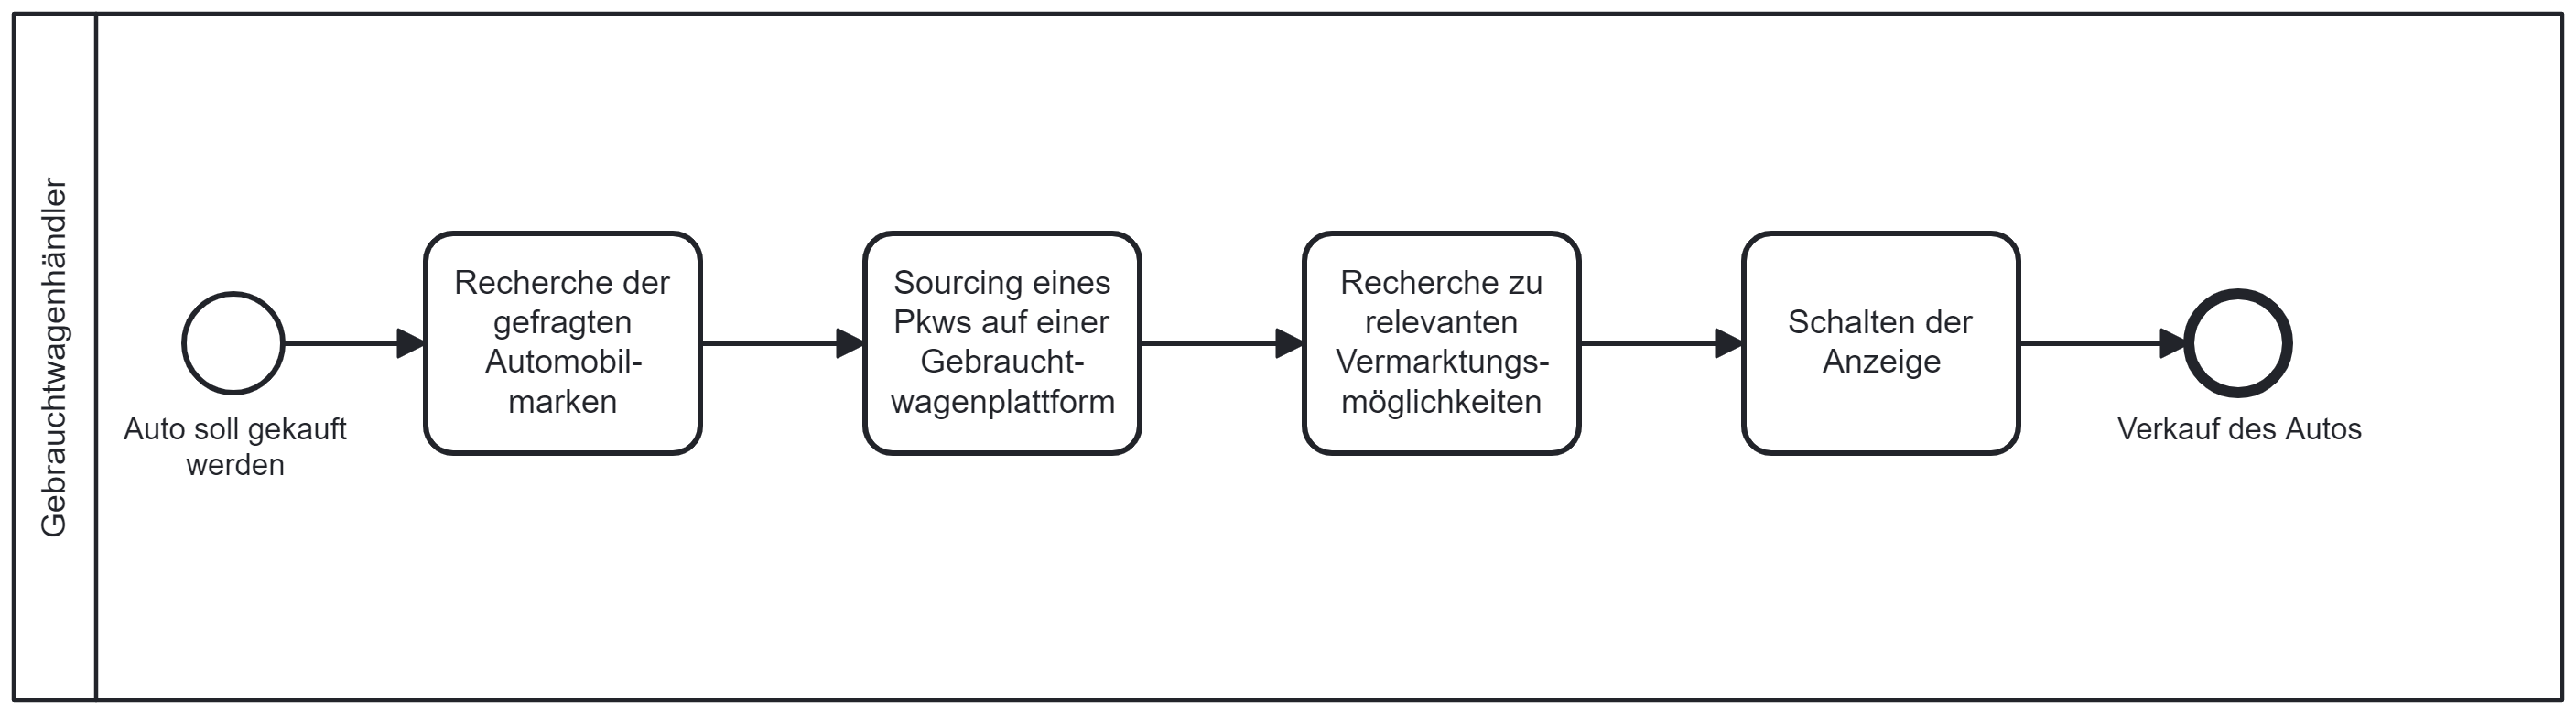
\includegraphics[width=\textwidth]{img/verkaufsprozess.png}
    \caption{Modellierung eines Geschäftsprozess eines Gebrauchtwagenhändlers mit Camunda Modeler}
    \label{fig:business-process}
\end{figure}
Anhand dieses Prozesses werden verschiedene Anwendungsfälle entwickelt, mit denen die Nützlichkeit der oben vorgestellten Visualisierungen erläutert werden soll: \\
\begin{itemize}
    \item Recherche einer relevanten Marke
    \item Recherche einer relevanten Anzeige
    \item Schalten einer optimierten Anzeige
\end{itemize}
\subsection{Starplot: Recherche einer relevanten Marke }

Ein Starplot bietet einem Gebrauchtwagenhändler eine leistungsstarke Möglichkeit, verschiedene Automarken zu analysieren und aufschlussreiche Erkenntnisse über durchschnittliche Werte in Bezug auf Preis, Leistung, Länge der Anzeige, Kilometerstand und Kraftstoffverbrauch zu gewinnen.  Zum Beispiel kann er Marken identifizieren, die im Vergleich zu anderen eine attraktive Kombination aus niedrigen durchschnittlichen Preisen, hoher Leistung, effizientem Kraftstoffverbrauch und moderater Laufleistung bieten. Das könnte zu potentiellen Wettbewerbsvorteilen führen. \\

Durch die visuelle Darstellung im Starplot wird die Vergleichbarkeit zwischen verschiedenen Marken vereinfacht, da der Händler auf einen Blick sehen kann, wie sich die durchschnittlichen Werte in den verschiedenen Kategorien unterscheiden. Dies ermöglicht es ihm,  Entscheidungen zu treffen und sein Inventar sowie Marketingstrategien besser auf die Bedürfnisse seiner Zielgruppe abzustimmen. Insgesamt bietet der Starplot eine effektive Möglichkeit, relevante Marken zu identifizieren und die Wettbewerbsposition des Gebrauchtwagenhändlers zu stärken. \\

\subsection{Scatterplot: Recherche einer relevanten Anzeige }

\begin{figure}[H]
    \centering
    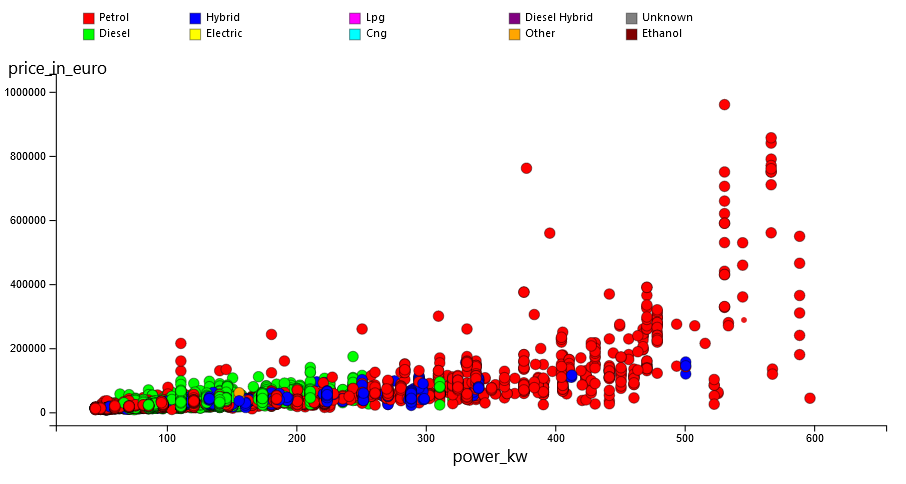
\includegraphics{img/anwendung2.png}
    \caption{Anwendungsfall 2}
    \label{fig:aw2}
\end{figure}

Gebrauchtwagenhänler müssen - ob auf Basis eines Kundenauftrags oder um ihr Portfolio zu erweitern - ständig relevante Anzeigen identifizieren.\\
Ein Gebrauchtwagenhändler kann mithilfe eines Scatterplots, bei dem die x-Achse die Leistung in Kilowatt (power\_kw) und die y-Achse den Preis in Euro (price\_in\_euro) darstellt, relevante Informationen aus Gebrauchtwagenanzeigen extrahieren. Diese Art der Datenvisualisierung bietet mehrere Vorteile für diesen Anwendungsfall. Der Scatterplot ermöglicht eine intuitive und leicht verständliche Darstellung der Beziehung zwischen Leistung und Preis für Gebrauchtwagen. Durch die  Anordnung der Datenpunkte im Scatterplot kann der Händler schnell Muster und Trends erkennen. \\

Die Leistung eines Fahrzeugs ist oft ein entscheidender Faktor für potenzielle Käufer, insbesondere in Bezug auf die  Effizienz. Durch die Visualisierung dieser Leistung im Zusammenhang mit dem Preis können Gebrauchtwagenhändler schnell Fahrzeuge identifizieren, die möglicherweise ein besonders attraktives Preis-Leistungs-Verhältnis bieten. Auf einen Blick lassen sich teure Fahrzeuge mit geringer Leistung oder preisgünstige Modelle mit überdurchschnittlicher Leistung erkennen. Dies erleichtert die Identifikation von Fahrzeugen, die sowohl den Leistungsforderungen als auch dem Budget der potenziellen Kunden entsprechen. Insgesamt unterstützt der Scatterplot als Datenvisualisierungsinstrument den Gebrauchtwagenhändler dabei, fundierte Entscheidungen zu treffen, das Sortiment zu optimieren und die Kundenbedürfnisse besser zu verstehen. \\

\subsection{Parallelplot: Schalten einer optimierten Anzeige}

Ein Parallelplot bietet einem Gebrauchtwagenhändler eine wirkungsvolle Methode, um relevante Anzeigen für bereits gekaufte Pkw zu schalten. Durch die Auswahl unterschiedlicher Parameter, insbesondere der Länge der Angebotsbeschreibung (length\_offer\_description) und des Sentiment-Scores der Angebotsbeschreibung (sentiment\_score), kann der Händler gezielt nach Anzeigen suchen, die gut zu den bereits erworbenen Fahrzeugen passen. \\

Die Länge der Angebotsbeschreibung kann ein Indikator für detaillierte und informative Anzeigen sein, die potenzielle Käufer ansprechen. Ein hoher Sentiment-Score deutet auf positiv formulierte Anzeigen hin, die das Interesse der Käufer wecken können. Durch die Auswahl dieser beiden Parameter als Hauptachsen im Parallelplot erhält der Händler einen visuellen Überblick über Anzeigen, die sowohl ausführlich als auch positiv formuliert sind. \\

Die Interaktivität des Parallelplots, insbesondere die Möglichkeit des Hovern, ermöglicht es dem Händler, bei Bedarf zusätzliche Informationen abzurufen. Durch Hovern über die Angebotsbeschreibung (offer\_description) kann er den genauen Text der Anzeige anzeigen lassen. Dies erleichtert die schnelle Identifizierung von Anzeigen, die die gewünschten Kriterien erfüllen, und ermöglicht dem Händler, gezielt relevante Anzeigen für bereits gekaufte Pkw zu schalten. \\

Insgesamt unterstützt der Parallelplot den Gebrauchtwagenhändler dabei, seine Marketingstrategie zu optimieren, indem er Anzeigen auswählt, die gut zu seinem bestehenden Inventar passen und die potenziellen Käufern klare und ansprechende Informationen bieten. Durch die visuelle Darstellung der Daten im Parallelplot kann der Händler Muster erkennen und so effektivere Entscheidungen für die Schaltung zielgerichteter Anzeigen treffen. \\